%-*- coding: utf-8 -*-
\textcolor[RGB]{46, 116, 181}{\chapter{Initialisation}}
Quelle que soit l’importance des avancées scientifiques et technologiques, c’est le travail des
professionnels de santé qui détermine la qualité et l’efficacité des soins. Dans ce contexte, les soins
nutritionnels, qui portent sur l’évaluation de l’état nutritionnel et l’accompagnement alimentaire des
patients hospitalisés, en interaction étroite avec l’équipe de soin, ne font pas exception. Pour ce
faire, les diététiciens développent des actions de complexité variable, tant au niveau des services de
soins que du système de restauration.

Simultanément, les professionnels doivent faire face à de nouveaux défis, dus aux modifications des
profils épidémiologiques, démographiques et sociaux des populations, ce qui exige la mise en place
de nouvelles compétences et la reconfiguration des stratégies d’action. Pour les diététiciens du
secteur hospitalier, elles ont pour conséquences de nouvelles exigences mentales et surtout
cognitives.

Le niveau de développement industriel de la filière alimentaire française allège la charge de travail
technique des diététiciens, non seulement en ce qui concerne la diversité de matières premières,
mais également dans le domaine du contrôle \enquote{qualité}, tout au long de la chaîne de production. De
la même façon, les nouveaux concepts de production en restauration collective, caractérisés par
l’utilisation de produits pré élaborés et l’innovation technologique des équipements, gagnent
visiblement du terrain dans le secteur hospitalier français.

\section{Définition du problème}
L'élaboration de menus dans un hôpital pour la restauration des patients
est une tâche complexe, et doit tenir compte des différentes pathologies
rencontrées. Faute de moyens (temps et argent) seules quelques grandes
lignes de restauration sont retenues; alors qu'idéalement, chaque
patient devrait pourvoir avoir un repas adapté à sa pathologie.

\section{Vision du projet}
\subsection{Solution envisagée}
Le projet Vitameal a pour objectif de faire correspondre au mieux la planification des régimes et des
prescriptions diététiques aux repas réellement servis au patient. Il consiste en un outil interfaçant la
gestion de production, la prise de commande et le suivi nutritionnel des repas.

\subsection{Périmètre}
C'est un diététicien qui renseigne le profil diététique des patients,
sous les directives des médecins. C'est aussi un diététicien qui élabore
les menus des patients. L'outil élaborera donc
les menus par filtrage des produits correspondants aux profils
diététiques des patients. Pour des raisons de simplifications, nous nous limiterons dans ce projet aux seuls patients adolescents et adultes.
\begin{figure}[H]
\label{Modelisation_du _probleme}
  \centering
      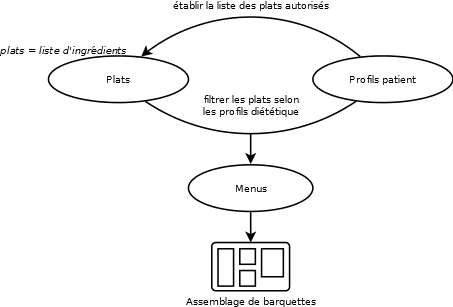
\includegraphics[width=0.75\textwidth]{problem_model} %
\caption{Modélisation du problème}
\end{figure}

\section{Analyse des exigences}
\subsection{Partie prenantes}
\begin{itemize}
\item Participantes~: les diététiciens, le service restauration
\item Concernés~: les médecins, la direction (budget)
\item Impactées~: les patients
\end{itemize}

\subsection{Les besoins}
En tant que diététicien, j’ai besoin de :
\begin{itemize}
 \item pouvoir renseigner le profil diététique des patients, pour qu’ils puissent bénéficier de menus adaptés.
 \item pouvoir élaborer les menus des 3 repas journaliers (petit-déjeuner, déjeuner et dîner), pour que ce soit fait automatiquement.
 \item pouvoir saisir des plats et leur composition, pour permettre l’émission d’une liste d’ingrédients à commander.
 \item élaborer des menus selon les fréquences de services du document R1 Annexes 2 et 4.
 \item classer chaque aliment dans une des catégories d’aliments citée dans les tables de grammages du document R1 Annexes 2 et 4.
\end{itemize}
En tant qu’administrateur du site internet de l’hôpital, j’ai besoin de récupérer le menu de la semaine, pour pouvoir l’afficher.

En tant que médecin, j’ai besoin de consulter les profils diététiques des patients admis, pour les  valider.

En tant que cuisiner du service restauration, j’ai besoin de consulter les menus élaborés, afin de pouvoir les préparer et de prévoir les ingrédients à commander.

En tant qu’agent de restauration hospitalière,  j’ai besoin de connaître les menus par patient, afin de pouvoir assembler les plateaux repas.

Les diététiciens renseignent les profils diététiques de chaque patient, sous les directives des médecins. Ils élaborent et planifient 3 menus par jours.

Les diététiciens ont besoin de saisir des plats avec les types d'aliments suivants:
\begin{itemize}
 \item céréalier (pain, biscottes, ou autre produit céréalier, …),
 \item laitier (lait, yaourt, fromage ou autre produit laitier, …)
 \item fruit (fruit cru, jus de fruit, compote, purée de fruit)
 \item lipidique (beurre, margarine, …)
 \item sucré (confiture, gelée, miel, …)
 \item protidique (jambon, oeuf, …)
\end{itemize}

Les diététiciens ont besoin d'élaborer les menus de chaque patient avec une quantité d'aliment correspondante au grammage de l'aliment pour sa tranche d'age (Document \ref{docNutrition}, Annexe 2). La fréquence de service de chaque aliment est conforme aux recommendations du document de nutrition \ref{docNutrition}, Annexe 4.

Le service restauration commande les produits et ingrédients mis en œuvre dans les menus, il prépare aussi les menus élaborés.

Le ditéticien élabore le petit déjeuner avec 1 boisson et 3 éléments principaux:
\begin{itemize}
 \item 1 boisson: eau, jus de fruit (100\% fruit), lait demi écrémé, café, thé, tisane ou chicorée. 
 \item 1 aliment céréalier
 \item 1 produit laitier (le lait est considéré comme une boisson et un produit laitier)
 \item 1 fruit (le jus de fruit est considéré comme une boisson et comme un fruit)
 \item complété selon type de population par:
 \begin{itemize}
  \item 1 élément lipidique (beurre, margarine, …)
  \item 1 élément sucré (confiture, gelée, miel, …)
  \item 1 élément protidique (jambon, oeuf, …)
 \end{itemize}
\end{itemize}

Lors de l'élaboration du petit déjeuner, le diététicien évite :
 \begin{itemize}
  \item les viennoiseries (croissant, pain au chocolat, …),
  \item les barres chocolatées,
  \item les biscuits chocolatés ou fourrés,
  \item les céréales fourrées,
  \item les pâtes à tartiner et les pâtisseries contenant plus de 15 \% de matières grasses \ref{docNutrition}, § 4.2.1.1.4 (page 39)
  \begin{itemize}
   \item Fréquence: 3 repas sur 20 au maximum
   \item pâtisseries comme
   \begin{itemize}
    \item les beignets,
    \item les viennoiseries,
    \item les gaufres,
    \item les crêpes fourrées au chocolat,
    \item les gâteaux à la crème ou au chocolat,
    \item les brownies au chocolat et aux noix,
    \item les quatre-quarts,
    \item les gâteaux moelleux chocolatés type napolitain mini-roulé,
    \item les biscuits chocolatés,
    \item les biscuits sablés nappés de chocolat,
    \item les biscuits secs chocolatés,
    \item les galettes ou les sablés,
    \item les goûters chocolatés fourrés,
    \item les gaufrettes fourrées,
    \item les madeleines,
    \item les biscuits secs feuilletés type palmier
    \item les cookies au chocolat.
   \end{itemize}
   \item autres desserts
   \begin{itemize}
    \item les tiramisus,
    \item les crèmes brûlées
    \item les glaces ou les nougats glacés.
   \end{itemize}
  \end{itemize}
 \end{itemize}

Le diététicien élabore les repas principaux avec 4 composantes, en plus du pain et de l'eau:
\begin{itemize}
 \item Entrées: Crudités, cuidités, entrées de légumes secs et ou d’autres féculents, entrées protidiques (oeuf, poisson), préparations pâtissières salées, charcuteries
 \item Plats protidiques: Plat principal à base de viande, poisson, oeuf, abats. Préparations pâtissières salées servies en plat principal (crêpes salées, friands divers, pizzas, tartes, quiches, tourtes). Charcuteries servies en plat principal (préparation traditionnelle à base de chair de porc, boudin noir, saucisses diverses, crépinettes, …).
 \item Garnitures: Légumes, légumes secs, pommes de terre, produits céréaliers.
 \item Produits laitiers: Lait demi-écrémé, lait fermenté ou autre produit laitier frais, fromage, dessert lacté.
 \item Desserts: Fruit crus entier ou en salade, fruit cuit ou au sirop, pâtisserie, biscuit, sorbet, dessert lacté, glace.
\end{itemize}

Le diététicien classe chaque aliment dans une des catégories d'aliments cité dans les tables de grammages et les fréquences de services du document \ref{docNutrition} Annexes 2 et 4.

Le diététicien, pour les personnes agées, tiens compte de leurs gouts et habitudes ainsi que de leur capacité de mastication $\rightarrow$ L’alimentation à texture modifiée, telle que viande moulinée ou purée de légumes, qui pourrait être proposée doit apporter au convive un apport protéino-énergétique suffisant. L’alimentation mixée ne comporte plus de pain. Cet apport énergétique doit être remplacé de façon quotidienne.

Le diététicien peut enrichir l'alimentation des personnes agées avec différents produits selon l'objectif attendu:
\begin{itemize}
 \item en protéines : avec du fromage, de la poudre de lait, du lait concentré, de l’oeuf, du jambon, du thon,… ;
 \item en calcium : avec des produits laitiers, fromage fondu dans les soupes, fromage râpé dans les plats,… ;
 \item en énergie : avec de la crème, beurre, lait concentré entier, crème de marrons,…
\end{itemize}

Le diététicien, pour satisfaire aux besoins protidiques et calciques des personnes âgées, enrichit les boissons lactées avec du lait en poudre à raison de 10\%. La boisson est d’au moins 150 ml de lait. Si la personne ne consomme pas de lait, on lui propose un laitage ou une portion de fromage.

Le diététicien élabore le petit déjeuner des personnes agées avec au moins 1/4 de la ration calorique nécessaire au quotidien. Ce repas comporte principalement :
\begin{itemize}
 \item une boisson en volume suffisant ($\ge 250 ml$) ;
 \item un aliment céréalier (pain, biscotte, pain de mie, céréales, ...) ;
 \item un produit laitier (lait, yaourt, fromage, fromage blanc, …) ;
 \item un fruit ou jus de fruit.
\end{itemize}
Pour ceux qui consomment peu de lait ($\le 150 ml$), il est remplacé par un autre produit laitier (yaourt, fromage, ....). Pour les personnes à risque de dénutrition ou dénutries, un enrichissement protidique et énergétique peut être proposé. Il peut comporter une ration protéique (jambon, oeuf, …).

Le diététicien élabore le déjeuner et le diner des personnes agées avec 5 composantes réparties comme suit, en plus du pain et d'une boison :
\begin{itemize}
 \item Entrées : crudités, cuidités, potages de légumes (minimum de 40 \% de légumes cuits, hors pommes de terres), potages de féculents, entrées de féculents ou légumes secs, entrées protidiques (charcuterie, poisson, oeuf), pâtisseries salées
 \item Soit
 \begin{itemize}
  \item Plats protidiques : viandes, abats, charcuteries, poissons, mollusques et crustacés, oeufs, plats composés à base de ces aliments
  \item Garnitures : légumes, légumes secs, légumineuses, pommes de terre, produits céréaliers
 \end{itemize}
 \item Soit: plat composé ou complet (cassoulet, choucroute, spaghetti bolognaise, hachis Parmentier, brandades Parmentier, … éviter les feuilletés, quiches, beignets, panés ou quenelles). Pour déterminer sa fréquence de service, on prend en compte le grammage de viande, poisson ou oeuf de la portion de plat complet servi.
 \item Produits laitiers dont fromages
 \item Desserts : fruits crus ou cuits, pâtisseries, entremets, crèmes desserts, sorbets et glaces.
\end{itemize}
Il veille à la présence de féculents dans les déjeuner et diner des personnes agées.

\subsection{Les contraintes}
\begin{itemize}
\item Les médecins doivent pouvoir vérifier / valider les profils diététiques des patients.
\item La direction fixe un budget maximum par menu.
\end{itemize}

\subsection{Exigences}
\begin{itemize}
\item Fonctionnelles
  \begin{itemize}
  \item Chaque patient a un profil diététique, renseigné par le diététicien
  \item Elaboration automatique des menus, correspondants à un ou plusieurs profils diététiques patients.
  \item À l'issue de l'élaboration des menus, la liste des produits et
    ingrédients (avec leur quantité) est faite afin que le service
    restauration puisse les commander.
  \item La liste des différents menus à réaliser (tickets patients), avec les quantités, est mise à disposition du service restauration pour faciliter l'assemblage du plateau repas.
  \item Ajout de plats.
  \item Chaque plat est décrit avec sa liste d'ingrédients, et la quantité nécessaire à sa réalisation par quantité de poids
  \item Planification des repas par cycles de X semaines
  \end{itemize}
%\item Non fonctionnelles
%  \begin{itemize}
%  \item \colorbox{yellow}{À évaluer !}
%  \end{itemize}
\end{itemize}

\section{\colorbox{yellow}{TODO} Estimation globale}
